% From the repository root, build with:
% latex -output-directory=/tmp assets/tex/grover_rotation.tex
% dvisvgm --no-fonts --exact --bbox=min -o assets/img/grover_rotation.svg /tmp/grover_rotation.dvi
\def\pgfsysdriver{pgfsys-dvisvgm.def}
\documentclass[tikz,border=6pt]{standalone}

\usepackage{amsmath}
\usetikzlibrary{arrows.meta, calc}

\begin{document}
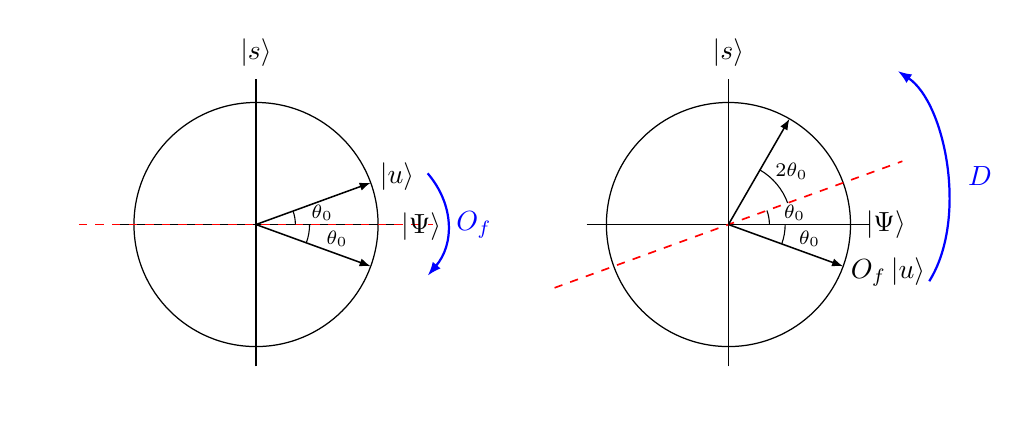
\begin{tikzpicture}[
  axis/.style={black, line width=0.45pt},
  state/.style={black, line width=0.55pt, -{Latex[length=4pt]}},
  reflection/.style={red, dashed, line width=0.6pt},
  operation/.style={blue, line width=0.8pt, -{Latex[length=5pt]}},
  angle mark/.style={black, line width=0.4pt},
  angle label/.style={font=\scriptsize, inner sep=1pt},
]
  \fill[white] (-5.9, -2.35) rectangle (6.4, 2.5);

  % Phase-oracle reflection.
  \coordinate (left) at (-3, 0);
  \draw[axis] (left) circle[radius=1.55];
  \draw[axis] (-3, -1.8) -- (-3, 1.85);
  \draw[axis] (-4.8, 0) -- (-1.2, 0);
  \draw[reflection] (-5.25, 0) -- (-0.75, 0);

  \draw[state] (left) -- ++(20:1.55);
  \draw[state] (left) -- ++(-20:1.55);

  \draw[angle mark] ($(left)+(0:0.50)$) arc[start angle=0, end angle=20, radius=0.50];
  \draw[angle mark] ($(left)+(-20:0.68)$) arc[start angle=-20, end angle=0, radius=0.68];

  \node[above] at (-3, 1.88) {$\left\lvert s\right\rangle$};
  \node[right] at (-1.55, 0.61) {$\left\lvert u\right\rangle$};
  \node[right] at (-1.28, -0.02) {$\left\lvert \Psi\right\rangle$};
  \node[angle label] at (-2.16, 0.15) {$\theta_0$};
  \node[angle label] at (-1.97, -0.18) {$\theta_0$};

  \draw[operation]
    (-0.82, 0.65) .. controls (-0.48, 0.25) and (-0.48, -0.25) .. (-0.82, -0.65);
  \node[blue, right] at (-0.58, 0) {$O_f$};

  % Grover diffusion reflection.
  \coordinate (right) at (3, 0);
  \draw[axis] (right) circle[radius=1.55];
  \draw[axis] (3, -1.8) -- (3, 1.85);
  \draw[axis] (1.2, 0) -- (4.8, 0);

  \draw[reflection] ($(right)+(200:2.35)$) -- ($(right)+(20:2.35)$);
  \draw[state] (right) -- ++(-20:1.55);
  \draw[state] (right) -- ++(60:1.55);

  \draw[angle mark] ($(right)+(-20:0.72)$) arc[start angle=-20, end angle=0, radius=0.72];
  \draw[angle mark] ($(right)+(0:0.52)$) arc[start angle=0, end angle=20, radius=0.52];
  \draw[angle mark] ($(right)+(20:0.80)$) arc[start angle=20, end angle=60, radius=0.80];

  \node[above] at (3, 1.88) {$\left\lvert s\right\rangle$};
  \node[right] at (4.62, 0) {$\left\lvert \Psi\right\rangle$};
  \node[right] at (4.43, -0.60) {$O_f\left\lvert u\right\rangle$};
  \node[angle label] at (4.03, -0.18) {$\theta_0$};
  \node[angle label] at (3.84, 0.15) {$\theta_0$};
  \node[angle label] at (3.80, 0.68) {$2\theta_0$};

  \draw[operation]
    (5.55, -0.72) .. controls (6.05, 0.08) and (5.75, 1.55) .. (5.15, 1.95);
  \node[blue, right] at (5.92, 0.62) {$D$};
\end{tikzpicture}
\end{document}
